% Author: Milos A. Saric, copyright 2025. https://saricmilos.com/

\title{Book Recommendation System --- Collaborative Filtering \& Content-Based Approaches}
\date{\today}
\author{Milos Saric}
\maketitle

% --------------- ABSTRACT
\begin{abstract}
This report investigates the Kaggle Book Recommendation dataset to develop intelligent book recommendation systems using both
collaborative filtering and content-based methods. A key application of machine learning is generating personalized recommendations
for users, aiming to boost revenue, engagement, or other performance metrics. As a result, understanding how these recommendation
algorithms work is an essential skill for anyone aspiring to become a Machine Learning Engineer.
Recommender systems have become a vital component of online platforms such
as YouTube, Amazon, and Netflix, helping users discover content tailored to their preferences. By analyzing user behavior and
item attributes, these systems predict user interests, enhancing user experience while driving engagement and revenue. 
This study highlights the implementation, advantages, and practical significance of recommendation algorithms in modern
digital platforms.
\end{abstract}

\rule{\linewidth}{0.5pt}

\section{Introduction and Problem Definition}

Recommender systems aim to predict user preferences and suggest items they are most likely to enjoy. This project focuses on developing a \textbf{book recommendation system} using the Kaggle \textbf{Book-Crossing Dataset}, leveraging both \textbf{collaborative filtering} and \textbf{content-based approaches} to deliver personalized book suggestions.
The goal is to design a system that accurately predicts and recommends books a user is likely to enjoy based on past interactions, ratings, and preferences. A clear understanding of this problem ensures that all subsequent analysis and modeling efforts align with the primary objective.


\begin{center}
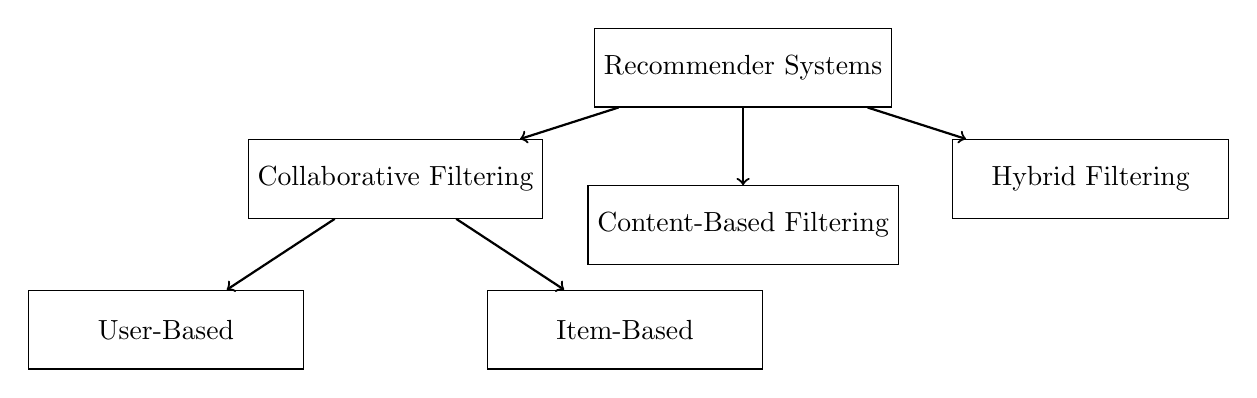
\begin{tikzpicture}[node distance=2cm, every node/.style={rectangle, draw, minimum width=3.5cm, minimum height=1cm, align=center}]
    % Nodes
    \node (RS) {Recommender Systems};
    \node (CF) [below left of=RS, xshift=-3cm] {Collaborative Filtering};
    \node (CB) [below of=RS] {Content-Based Filtering};
    \node (Hybrid) [below right of=RS, xshift=3cm] {Hybrid Filtering};
    \node (User) [below left of=CF, xshift=-1.5cm, yshift=-0.5cm] {User-Based};
    \node (Item) [below right of=CF, xshift=1.5cm, yshift=-0.5cm] {Item-Based};

    % Arrows
    \draw[->, thick] (RS) -- (CF);
    \draw[->, thick] (RS) -- (CB);
    \draw[->, thick] (RS) -- (Hybrid);
    \draw[->, thick] (CF) -- (User);
    \draw[->, thick] (CF) -- (Item);
\end{tikzpicture}
\end{center}

\subsection{Scope}
The analysis focuses exclusively on the Kaggle dataset, which includes:  
\begin{itemize}
    \item \textbf{Users:} demographic and identification data.  
    \item \textbf{Books:} metadata such as title, author, year, publisher, and cover images.  
    \item \textbf{Ratings:} explicit ratings (1--10) and implicit feedback (0 for interactions without ratings).  
\end{itemize}
Predictions are restricted to this dataset without using external sources unless explicitly integrated in advanced phases.

\subsection{Stakeholders}
\begin{itemize}
    \item \textbf{Readers / Users:} receive personalized book recommendations.  
    \item \textbf{Publishers / Authors:} gain insights into reader interests for better targeting.  
    \item \textbf{Data Scientists / ML Practitioners:} test and optimize recommendation algorithms.  
    \item \textbf{Platform Developers / Businesses:} improve user engagement, retention, and revenue through effective recommendations.
\end{itemize}


\section{Collaborative Filtering}
Collaborative filtering creates a model based on a user's past actions—such as items they have purchased, selected, or
rated, as well as the behavior of other users with similar preferences. This model is then used to recommend items or predict 
ratings for items that the user is likely to be interested in.
Collaborative filtering is a recommendation method that predicts a users preferences based on the choices of other users
with similar tastes. It relies on both user and item information, often organized in a user-item matrix.

This approach is widely used in industry across platforms like YouTube, Netflix, Amazon, and Medium. 
For example, if users with similar demographics buy a product on Amazon, the system can suggest that same product to you.
YouTube leverages this technique to recommend videos, Medium uses it to suggest articles, and Netflix relies heavily on
collaborative filtering to personalize movie recommendations.

\begin{center}
\begin{tikzpicture}[node distance=2.5cm, every node/.style={rectangle, draw, minimum width=2.5cm, minimum height=1cm, align=center}]

    % Users
    \node (User1) {User 1};
    \node (User2) [right=6cm of User1] {User 2};

    % Similarity label node
    \node[draw=none, fill=none] (SimilarLabel) [above=0.3cm of $(User1)!0.5!(User2)$] {similar};
    \draw[<->, thick] (User1) -- (User2);

    % Books for User1
    \node (Book1) [below=3cm of User1, xshift=-1.5cm] {1984};
    \node (Book2) [below=3cm of User1, xshift=1.5cm] {Steve Jobs};

    % Books for User2
    \node (Book3) [below=3cm of User2, xshift=-2.0cm] {1984};
    \node (Book4) [below=3cm of User2] {Steve Jobs};
    \node (Book5) [below=3cm of User2, xshift=2.0cm] {Stiff};

    % Arrows from User1 to books
    \draw[->, thick] (User1) -- (Book1);
    \draw[->, thick] (User1) -- (Book2);

    % Arrows from User2 to books
    \draw[->, thick] (User2) -- (Book3);
    \draw[->, thick] (User2) -- (Book4);
    \draw[->, thick] (User2) -- (Book5);

    % Recommendation arrow from Book5 to User1
    \node[draw=none, fill=none] (RecLabel) [right=1cm of Book5.north east] {recommend};
    \draw[->, thick, red] (Book5.north) -- ++(0,1) -| (User1.south);

\end{tikzpicture}
\end{center}

\begin{tikzpicture}[
    user/.style={rectangle, draw=none, fill=cyan!20, rounded corners, minimum width=1.6cm, minimum height=0.7cm, align=center},
    item/.style={rectangle, draw=none, fill=green!20, rounded corners, minimum width=1.6cm, minimum height=0.7cm, align=center},
    like/.style={-{Stealth}, thick},
    recommend/.style={-{Stealth}, thick, dashed, red},
    every node/.style={font=\small}
]

% Users
\node[user] (A) {User A};
\node[user, below=0.8cm of A] (B) {User B};
\node[user, below=0.8cm of B] (C) {User C};

% Items
\node[item, right=3.5cm of A] (IA) {item A};
\node[item, below=0.8cm of IA] (IB) {item B};
\node[item, below=0.8cm of IB] (IC) {item C};
\node[item, below=0.8cm of IC] (ID) {item D};

% Similarity label
\draw[-{Stealth}, thick] ($(A.west)+(-0.7,0)$) -- ++(0,-1.6) node[midway,left]{Similar};

% Like arrows (solid)
\draw[like] (A) -- (IA);
\draw[like] (A) -- (IB);
\draw[like] (B) -- (IB);
\draw[like] (B) -- (IC);
\draw[like] (C) -- (IC);
\draw[like] (C) -- (ID);

% Recommend arrows (dashed red)
\draw[recommend] (A) -- (IC);
\draw[recommend] (A) -- (ID);

% Legend
\node[above=0.5cm of A, align=left] (legend) {
\begin{tabular}{@{}ll@{}}
\raisebox{0.5ex}{\tikz{\draw[like] (0,0)--(0.6,0);}} & like \\
\raisebox{0.5ex}{\tikz{\draw[recommend] (0,0)--(0.6,0);}} & recommend
\end{tabular}
};

% Caption
\node[below=0.8cm of C] {\textbf{User-Based CF}};

\end{tikzpicture}


\begin{tikzpicture}[
    user/.style={rectangle, draw=none, fill=cyan!20, rounded corners, minimum width=1.6cm, minimum height=0.7cm, align=center},
    item/.style={rectangle, draw=none, fill=green!20, rounded corners, minimum width=1.6cm, minimum height=0.7cm, align=center},
    like/.style={-{Stealth}, thick},
    recommend/.style={-{Stealth}, thick, dashed, red},
    every node/.style={font=\small}
]

% Users
\node[user] (A) {User A};
\node[user, below=0.8cm of A] (B) {User B};
\node[user, below=0.8cm of B] (C) {User C};

% Items
\node[item, right=3.5cm of A] (IA) {item A};
\node[item, below=0.8cm of IA] (IB) {item B};
\node[item, below=0.8cm of IB] (IC) {item C};
\node[item, below=0.8cm of IC] (ID) {item D};

% Like arrows (solid)
\draw[like] (A) -- (IA);
\draw[like] (A) -- (IB);
\draw[like] (B) -- (IB);
\draw[like] (B) -- (IC);
\draw[like] (C) -- (IC);

% Recommend arrow (dashed red)
\draw[recommend] (C) -- (ID);

% Similarity between items (right side)
\draw[-{Stealth}, thick] (IA.east) -- ++(0.7,-2.4) node[midway,right]{Similar};

% Similarity arrow connecting items
\draw[like] (ID.east) -- ++(0.7,2.4);

% Legend
\node[above=0.5cm of A, align=left] (legend) {
\begin{tabular}{@{}ll@{}}
\raisebox{0.5ex}{\tikz{\draw[like] (0,0)--(0.6,0);}} & like \\
\raisebox{0.5ex}{\tikz{\draw[recommend] (0,0)--(0.6,0);}} & recommend
\end{tabular}
};

% Caption
\node[below=0.8cm of C] {\textbf{item-Based CF}};

\end{tikzpicture}

\begin{figure}[H]
    \centering
    % Left image
    \begin{subfigure}[b]{0.48\textwidth}
        \centering
        \includegraphics[width=\textwidth]{figures/collaborative_filter.PNG}
        \caption{User Based Collaborative Filtering}
        \label{fig:collaborative_filtering}
    \end{subfigure}
    \hfill
    % Right image
    \begin{subfigure}[b]{0.48\textwidth}
        \centering
        \includegraphics[width=\textwidth]{figures/user_item_based.PNG}
        \caption{User and Item Based Collaborative Filtering}
        \label{fig:user_item_based}
    \end{subfigure}
    
    \caption{Comparison of Collaborative Filtering Approaches}
    \label{fig:collab_side_by_side}
\end{figure}

In our book recommendation system, we begin by constructing a matrix with users as rows and books (identified by ISBN) as columns—let’s call this the user–book matrix.

Each entry in the matrix represents either a rating from 1 to 10, indicating that the user has read and rated the book,
or a zero if the user has not interacted with that book. For example, if user J has rated book K, the corresponding cell
contains that rating. If user J has not read or rated book K, the cell is simply zero.

\subsection{User-Based Collaborative Filtering}

User-based collaborative filtering recommends items to a user by identifying other users with similar preferences. If a similar user liked an item, it can be suggested. 

\subsubsection{Cosine similarity with top-K neighbors}

Similarity between users can be measured using metrics such as \textbf{Cosine similarity}, \textbf{Pearson correlation}, or \textbf{Euclidean distance}.

The predicted rating $\hat{r}_{u,i}$ of user $u$ for item $i$ can be calculated as:

\begin{equation}
\hat{r}_{u,i} = \frac{\sum_{v \in N(u)} s(u,v) \cdot r_{v,i}}{\sum_{v \in N(u)} |s(u,v)|}
\end{equation}

where:  
\begin{itemize}
    \item $N(u)$ is the set of users similar to user $u$,  
    \item $s(u,v)$ is the similarity between users $u$ and $v$,  
    \item $r_{v,i}$ is the rating given by user $v$ to item $i$.  
\end{itemize}

In short, the predicted rating is a weighted average of ratings from similar users, with weights determined by user similarity.

User-based collaborative filtering predicts a user's rating for an item based on the ratings of similar users. The steps are:

\begin{enumerate}
    \item Represent each user as a vector in item space:
    \[
    \mathbf{u}_i = [r_{i1}, r_{i2}, r_{i3}, \dots, r_{iM}]
    \]
    where \(r_{ij}\) is the rating of user \(i\) for item \(j\), and \(M\) is the number of items.
    
    \item Compute user-user similarity, e.g., using \textbf{cosine similarity}:
    \begin{equation}
    \text{sim}(u, v) = \frac{\mathbf{u} \cdot \mathbf{v}}{\|\mathbf{u}\| \, \|\mathbf{v}\|}
    \end{equation}
    where \(\mathbf{u} \cdot \mathbf{v}\) is the dot product, and \(\|\mathbf{u}\|\) is the Euclidean norm:
    \begin{equation}
    \|\mathbf{u}\| = \sqrt{\sum_{j=1}^{M} r_{uj}^2}
    \end{equation}
    
    \item Predict ratings for a user \(u\) on item \(i\) using top-K similar users \(N(u)\):
    \begin{equation}
    \hat{r}_{ui} = \bar{r}_u + \frac{\sum_{v \in N(u)} \text{sim}(u,v) (r_{vi} - \bar{r}_v)}{\sum_{v \in N(u)} |\text{sim}(u,v)|}
    \end{equation}
    where \(\bar{r}_u\) is the mean rating of user \(u\).
\end{enumerate}

\subsection*{Intuition of Cosine Similarity}

\begin{itemize}
    \item Each user is a vector in \(M\)-dimensional space, where each axis represents an item.
    \item The length of the vector corresponds to the magnitude of their ratings.
    \item Cosine similarity measures the \textbf{angle between user vectors}, i.e., the similarity in rating patterns.
    \item Example:

\[
\text{User A} = [5, 3, 0], \quad
\text{User B} = [4, 2, 0]
\]

Even though User B gives slightly lower ratings, the \textit{pattern is similar}, resulting in a high cosine similarity.
\end{itemize}



\tdplotsetmaincoords{60}{120}
\begin{center}
\begin{tikzpicture}[tdplot_main_coords, scale=2]

% Draw axes
\draw[->] (0,0,0) -- (1.2,0,0) node[anchor=north east]{$\text{Item 1}$};
\draw[->] (0,0,0) -- (0,1.2,0) node[anchor=north west]{$\text{Item 2}$};
\draw[->] (0,0,0) -- (0,0,1.2) node[anchor=south]{$\text{Item 3}$};

% Draw user vectors
\draw[->, thick, blue] (0,0,0) -- (1,0.6,0) node[midway, above] {User A};
\draw[->, thick, red] (0,0,0) -- (0.8,0.4,0) node[midway, above right] {User B};
\draw[->, thick, green] (0,0,0) -- (0.2,1,0.6) node[midway, right] {User C};

% Optionally draw angle between A and B
\draw[dashed] (0,0,0) -- (1,0.6,0);
\draw[dashed] (0,0,0) -- (0.8,0.4,0);

\end{tikzpicture}
\end{center}

Cosine similarity compares rating patterns, not absolute rating levels.
Length of the vector = total “strength” of user ratings, but cosine similarity is normalized so that only direction matters.

\section{User-Based Collaborative Filtering: Vector Representation}

\subsection{From Ratings to Vectors}

In user-based collaborative filtering, we start from a set of observed user--item ratings
\[
R = \{(u, i, r_{ui}) \mid u \in U,\, i \in I \}
\]
where $U$ is the set of users, $I$ is the set of items (books), and $r_{ui}$ is the rating given by user $u$ to item $i$.

We represent this data as a \textbf{user--item rating matrix} $M \in \mathbb{R}^{|U| \times |I|}$:
\[
M_{ui} =
\begin{cases}
r_{ui}, & \text{if user } u \text{ rated item } i \\
0, & \text{otherwise.}
\end{cases}
\]

Each \textbf{row} of this matrix corresponds to a \emph{user vector}:
\[
\mathbf{u}_k = [\, r_{k1}, r_{k2}, \ldots, r_{k|I|} \,] \in \mathbb{R}^{|I|}
\]
Thus, the moment we pivot our data from a triplet $(u, i, r_{ui})$ format into a matrix form,
we have implicitly constructed a high-dimensional vector representation for every user.

\subsection{User Similarity Computation}

To measure the similarity between two users $u$ and $v$, we use cosine similarity:
\[
\text{sim}(u, v) = 
\frac{\mathbf{u}_u \cdot \mathbf{u}_v}
     {\|\mathbf{u}_u\|_2 \, \|\mathbf{u}_v\|_2}
= \frac{\sum_{i \in I} r_{ui} r_{vi}}
       {\sqrt{\sum_{i \in I} r_{ui}^2} \sqrt{\sum_{i \in I} r_{vi}^2}}
\]

The cosine similarity compares the orientation of two users’ rating vectors in the item space.
If two users rated similar items similarly, their vectors will point in nearly the same direction,
yielding a high cosine similarity.

\subsection{Prediction Step}

For an active user $u$ and target item $i$, we predict the rating $\hat{r}_{ui}$ as a weighted average of ratings from similar users:
\[
\hat{r}_{ui} =
\frac{\sum_{v \in N_u} \text{sim}(u, v) \, r_{vi}}
     {\sum_{v \in N_u} |\text{sim}(u, v)|}
\]
where $N_u$ is the set of top-$k$ most similar users to $u$ who have rated item $i$.

\subsection{Example of User Vectors}

Consider three users and four items:

\[
M =
\begin{bmatrix}
5 & 0 & 3 & 0 \\
4 & 2 & 0 & 0 \\
0 & 0 & 4 & 5
\end{bmatrix}
\]

This corresponds to the following user vectors:
\[
\mathbf{u}_1 = [5, 0, 3, 0], \quad
\mathbf{u}_2 = [4, 2, 0, 0], \quad
\mathbf{u}_3 = [0, 0, 4, 5]
\]

Each user is now represented as a point in a 4-dimensional space
(1 dimension per item). Similarities are computed between these vectors.

\subsection{Illustration in Vector Space}

\begin{center}
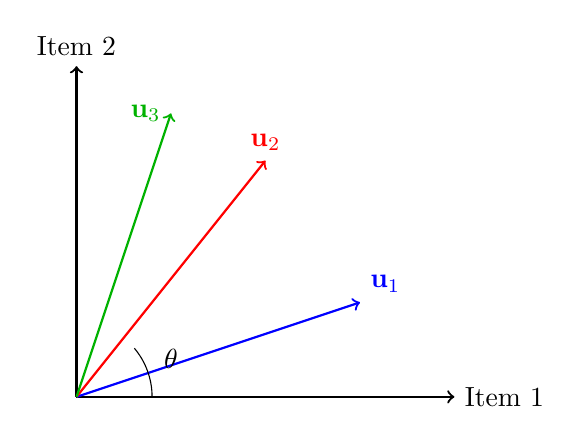
\begin{tikzpicture}[scale=1.2]
    % Axes
    \draw[->, thick] (0,0) -- (4,0) node[right] {Item 1};
    \draw[->, thick] (0,0) -- (0,3.5) node[above] {Item 2};

    % User vectors
    \draw[->, thick, blue] (0,0) -- (3,1) node[above right] {$\mathbf{u}_1$};
    \draw[->, thick, red] (0,0) -- (2,2.5) node[above] {$\mathbf{u}_2$};
    \draw[->, thick, green!70!black] (0,0) -- (1,3) node[left] {$\mathbf{u}_3$};

    % Angle between u1 and u2
    \draw (0.8,0) arc[start angle=0,end angle=40,radius=0.8];
    \node at (1.0,0.4) {$\theta$};
\end{tikzpicture}
\end{center}

In this simplified 2D example (only two items), each user is a vector
in the \emph{item space}. The angle $\theta$ between two users
represents their dissimilarity, while $\cos(\theta)$ represents their similarity.

\subsection{Summary}

\begin{itemize}
    \item Each user is a vector in an $|I|$-dimensional space (items are dimensions).
    \item Ratings are vector components (coordinate values).
    \item Similarities are computed between users’ vectors.
    \item Predictions are weighted averages of neighbors’ ratings.
\end{itemize}

\subsection{User-Based vs. Item-Based Cosine Similarity}

The cosine similarity function itself does not know whether we are computing
user-based or item-based similarity. The distinction depends solely on the orientation
of the rating matrix $M$.

Given the rating matrix
\[
M_{ui} =
\begin{bmatrix}
5 & 3 & 0 \\
4 & 0 & 2 \\
0 & 4 & 5
\end{bmatrix},
\]
we have two perspectives:

\begin{enumerate}
    \item \textbf{User-Based Filtering:}
    Each user is represented as a vector in the \emph{item space}.
    Similarity is computed between rows:
    \[
    \text{sim}(u, v) = 
    \frac{M_u \cdot M_v}
         {\|M_u\|\|M_v\|}.
    \]
    This yields a user--user similarity matrix of shape $|U| \times |U|$.

    \item \textbf{Item-Based Filtering:}
    Each item is represented as a vector in the \emph{user space}.
    Similarity is computed between columns:
    \[
    \text{sim}(i, j) =
    \frac{M^T_i \cdot M^T_j}
         {\|M^T_i\|\|M^T_j\|}.
    \]
    This yields an item--item similarity matrix of shape $|I| \times |I|$.
\end{enumerate}

In practice, this difference is implemented by transposing the matrix before applying
cosine similarity:
\[
\text{user-based: } \text{cosine\_similarity}(M), \quad
\text{item-based: } \text{cosine\_similarity}(M^T).
\]

\subsection{Item-Based Collaborative Filtering}

Item-based collaborative filtering recommends items by analyzing their similarity based on user interactions. 
In other words, if two items receive similar ratings from many users, they are considered similar. 
For instance, Amazon can suggest a product based on items with similar user ratings,
Netflix can recommend a movie or Goodreads can recommend an book based on other books with similar engagement patterns.

To compute the similarity between items, we often use metrics such as \textbf{Cosine similarity}, applied to the user-item matrix along the item dimension. Once the item-item similarity matrix is created, the predicted rating $\hat{r}_{u,i}$ for user $u$ on item $i$ can be computed as:

\begin{equation}
\hat{r}_{u,i} = \frac{\sum_{j \in N(i)} s(i,j) \cdot r_{u,j}}{\sum_{j \in N(i)} |s(i,j)|}
\end{equation}

where:  
\begin{itemize}
    \item $N(i)$ is the set of items similar to item $i$,  
    \item $s(i,j)$ is the similarity between items $i$ and $j$,  
    \item $r_{u,j}$ is the rating of user $u$ for item $j$.  
\end{itemize}

This formula is analogous to user-based collaborative filtering, but here the weights come from item-item similarity instead of user-user similarity.  

The quality of predictions can be evaluated using metrics like \textbf{Mean Squared Error (MSE)} or other regression metrics.

Item-based collaborative filtering predicts a user's rating for an item based on ratings of \textbf{similar items} that the user has already rated.

\subsection*{Steps}

\begin{enumerate}
    \item Represent each item as a vector in user space:
    \[
    \mathbf{i}_j = [r_{1j}, r_{2j}, r_{3j}, \dots, r_{Nj}]
    \]
    where \(r_{uj}\) is the rating user \(u\) gave to item \(j\), and \(N\) is the number of users.

    \item Compute an item–item similarity matrix using cosine similarity:
    \[
    \text{sim}(i, j) = \frac{\mathbf{i}_i \cdot \mathbf{i}_j}{\|\mathbf{i}_i\| \, \|\mathbf{i}_j\|}
    \]

    \item Predict a user \(u\)'s rating for item \(j\) using similar items they have rated:
    \[
    \hat{r}_{uj} = \frac{\sum_{k \in N(j)} \text{sim}(j,k) \cdot r_{uk}}{\sum_{k \in N(j)} |\text{sim}(j,k)|}
    \]
    where \(N(j)\) is the set of top-K similar items to \(j\) that the user has rated.
\end{enumerate}

\subsection*{Intuition}

\begin{itemize}
    \item Each item is a vector in \(N\)-dimensional user space.
    \item Cosine similarity measures which items are rated similarly by users.
    \item Works well in sparse datasets because items tend to have more ratings than individual users.
\end{itemize}

\subsection*{Graphical Illustration}

\tdplotsetmaincoords{60}{120}
\begin{tikzpicture}[tdplot_main_coords, scale=2]

% Draw axes
\draw[->] (0,0,0) -- (1.2,0,0) node[anchor=north east]{$\text{User 1}$};
\draw[->] (0,0,0) -- (0,1.2,0) node[anchor=north west]{$\text{User 2}$};
\draw[->] (0,0,0) -- (0,0,1.2) node[anchor=south]{$\text{User 3}$};

% Draw item vectors
\draw[->, thick, blue] (0,0,0) -- (1,0.6,0) node[midway, above] {Item A};
\draw[->, thick, red] (0,0,0) -- (0.8,0.4,0) node[midway, above right] {Item B};
\draw[->, thick, green] (0,0,0) -- (0.2,1,0.6) node[midway, right] {Item C};

% Optionally dashed lines for visual reference
\draw[dashed] (0,0,0) -- (1,0.6,0);
\draw[dashed] (0,0,0) -- (0.8,0.4,0);

\end{tikzpicture}

\subsection{Comparison of User-Based and Item-Based Collaborative Filtering}

User-item matrices are typically very sparse, meaning that most users interact with only a small fraction of available items. This sparsity affects both computational complexity and recommendation behavior.

\subsubsection{User-Based Filtering}
User-based collaborative filtering can offer more diverse recommendations because it focuses on similarities between users rather than items. For example, if user X likes an item that user J has never seen, user J may still receive a recommendation for that item if their overall preferences are similar. The main drawback is computational cost: calculating the K nearest neighbors for each user can be expensive.

\subsubsection{Item-Based Filtering}
Item-based filtering often seems more computationally intensive, but much of the work can be done offline. Specifically, the item–item similarity matrix can be precomputed because items change less frequently than users. This reduces repeated calculations but can lead to less diverse recommendations, as items similar to those already liked are more likely to be suggested.

\subsection{Data Dependency and Model Adaptation}

Collaborative filtering relies heavily on user data. As users continue to browse, purchase, and rate products, their preferences evolve over time. Because of this, the underlying recommendation model must be regularly updated and refined to stay accurate and relevant. In practice, this means continuously integrating new data and adjusting the system to reflect changing user behavior and market trends.

The two main sources of data for collaborative filtering are:

\begin{itemize}
    \item \textbf{Explicit data:} Information that users actively provide, such as ratings, reviews, or responses to surveys and questionnaires.
    \item \textbf{Implicit data:} Information inferred from user behavior, including browsing history, clicks, time spent on content, likes, shares, and other engagement signals.
\end{itemize}

Both types of data are essential for understanding user preferences. Explicit ratings capture direct feedback, while implicit data reveals natural behavioral patterns that help improve recommendation accuracy over time.

\section{Content Based Filtering}


Content-based filtering is one of the two primary approaches in recommender systems.  
It generates recommendations by analyzing the features of items and matching them to a user's preferences. Essentially, the system compares a \textbf{user profile} with an \textbf{item profile} to predict which items the user is likely to engage with.
Content-Based Recommender Systems (CBRSs) often build a personalized model for each user. The process begins by collecting the features of items the user has interacted with—this forms the user profile. These items serve as a training set for a user-specific classifier or regression model. 

In the model, the item features act as independent variables, while the user's past behavior-such as ratings, likes, 
or purchases—serves as the dependent variable. Once trained, the model predicts the user's likely response to new items, 
allowing the system to recommend items that align with the user's preferences.
The \textbf{item profile} captures the characteristics of an item, including structured features or descriptive metadata. For example, a streaming service may represent movies using attributes such as genre, director, release year, or cast.  

The \textbf{user profile} reflects the individual's preferences and past behavior. It is typically built from items the user has previously interacted with, including ratings, likes, dislikes, searches, or other engagement data.  

Content-based recommender systems often incorporate machine learning and data science techniques to improve prediction accuracy, enabling the recommendation of new items that match the user’s interests.  
In short, this approach focuses on \textit{what the user likes}, rather than what other users like.

\subsection{Item Representations in Content-Based Filtering}

In content-based filtering, items and users are often represented as vectors in a multi-dimensional feature space. Each item's feature—such as genre, author, or other metadata—define its coordinates. Boolean values (1 for presence, 0 for absence) are commonly used to indicate whether an item possesses a particular feature.

\textbf{Example:} A few novels represented by three genres (Adventure, Bildungsroman, Children):

\begin{table}[H]
\centering
\caption{Boolean Feature Representation of Novels}
\begin{tabular}{|l|c|c|c|}
\hline
\textbf{Novel} & \textbf{Adventure} & \textbf{Bildungsroman} & \textbf{Children} \\
\hline
Little Women & 0 & 1 & 1 \\
Northanger Abbey & 0 & 1 & 0 \\
Peter Pan & 1 & 0 & 1 \\
Treasure Island & 1 & 0 & 1 \\
\hline
\end{tabular}
\end{table}

In this 3D vector space, each dimension corresponds to a feature (Adventure, Bildungsroman, Children). A novel’s coordinates are determined by its Boolean values. For example:

\begin{itemize}
    \item \textit{Little Women:} (0,1,1)  
    \item \textit{Northanger Abbey:} (0,1,0)  
    \item \textit{Peter Pan:} (1,0,1)  
    \item \textit{Treasure Island:} (1,0,1)  
\end{itemize}

% Set up 3D coordinates
\tdplotsetmaincoords{70}{120} % Adjust viewing angle

\begin{center}
\begin{tikzpicture}[scale=3,tdplot_main_coords]
    % Axes
    \draw[->] (0,0,0) -- (1.5,0,0) node[anchor=north east] {Bildungsroman (X)};
    \draw[->] (0,0,0) -- (0,1.5,0) node[anchor=south west] {Adventure (Y)};
    \draw[->] (0,0,0) -- (0,0,1.5) node[anchor=south] {Children's Literature (Z)};
    
    % Plot novels
    \coordinate (LW) at (0,1,1);
    \coordinate (NA) at (0,1,0);
    \coordinate (PP) at (1,0,1);
    \coordinate (TI) at (1,0,1);
    
    % Draw points
    \filldraw[red] (LW) circle (0.03) node[above right] {Little Women};
    \filldraw[blue] (NA) circle (0.03) node[below right] {Northanger Abbey};
    \filldraw[green] (PP) circle (0.03) node[above left] {Peter Pan};
    \filldraw[orange] (TI) circle (0.03) node[below left] {Treasure Island};
    
    % Optional: dashed lines to axes for clarity
    \draw[dashed, gray] (LW) -- (0,1,0) -- (0,0,0);
    \draw[dashed, gray] (NA) -- (0,0,0);
    \draw[dashed, gray] (PP) -- (1,0,0) -- (0,0,0);
    \draw[dashed, gray] (TI) -- (1,0,0) -- (0,0,0);
\end{tikzpicture}
\end{center}

The closer two novels are in this space, the more similar they are according to the selected features. For instance,
 \textit{Peter Pan} and \textit{Treasure Island} overlap completely, while \textit{Little Women} is closer to
  \textit{Northanger Abbey} than to the adventure novels.  Since Peter Pan and Treasure Island are very similar in the feature space,
   a user who has previously purchased Peter Pan is likely to be recommended Treasure Island, as it closely matches their interests.

\textbf{Visualization:} We can plot these items in a 3D Cartesian coordinate system, with each axis representing one genre. Novel vectors are points in this space, and proximity reflects similarity. Adding more features (e.g., Fantasy, Gothic) increases the dimensionality, adjusting item positions accordingly.

\subsection{Similarity Metrics}

\subsubsection{Cosine Similarity}

In content-based filtering, the system determines how similar two items are by comparing their feature representations in the vector space. Items that are closer together are considered more alike, and this similarity can be measured using various metrics.

One of the most common methods, especially for high-dimensional feature spaces, is \textbf{Cosine Similarity}. Cosine similarity measures the angle between two vectors, giving a value between -1 and 1. The closer the value is to 1, the more similar the items are considered. 

The formula for cosine similarity between two item vectors $\mathbf{x}$ and $\mathbf{y}$ is:

\begin{equation}
\text{sim}(\mathbf{x}, \mathbf{y}) = \frac{\mathbf{x} \cdot \mathbf{y}}{\|\mathbf{x}\| \, \|\mathbf{y}\|} 
= \frac{\sum_{i=1}^{n} x_i y_i}{\sqrt{\sum_{i=1}^{n} x_i^2} \; \sqrt{\sum_{i=1}^{n} y_i^2}}
\end{equation}

Here, $\mathbf{x} \cdot \mathbf{y}$ represents the dot product of the two vectors, and $\|\mathbf{x}\|$ and $\|\mathbf{y}\|$ are the magnitudes (lengths) of the vectors. This metric allows the system to quantify similarity between items and recommend those that are most closely aligned with the user's previous preferences.

where $\mathbf{x}$ and $\mathbf{y}$ are vectors, for example, item feature vectors in a recommendation system.  

\begin{itemize}
    \item The \textbf{dot product} $\mathbf{x} \cdot \mathbf{y}$ quantifies how much the two vectors point in the same direction.
    \item The \textbf{norms} $\|\mathbf{x}\|$ and $\|\mathbf{y}\|$ normalize the vectors by their lengths.
\end{itemize}

The result ranges from $-1$ to $1$, where values closer to $1$ indicate highly similar items, and values near $0$ indicate little similarity.  

Cosine similarity can be understood geometrically as the cosine of the angle $\theta$ between two vectors:

\begin{equation}
\text{sim}(\mathbf{x}, \mathbf{y}) = \cos \theta
\end{equation}

\begin{center}
\begin{tikzpicture}[scale=2]
    % Draw axes
    \draw[->] (0,0) -- (2,0) node[right] {$x$};
    \draw[->] (0,0) -- (0,2) node[above] {$y$};

    % Draw vectors
    \draw[->, thick, blue] (0,0) -- (1.5,1) node[midway, above] {$\mathbf{x}$};
    \draw[->, thick, red] (0,0) -- (1,1.5) node[midway, left] {$\mathbf{y}$};

    % Draw angle theta
    \draw (0.5,0) arc (0:34.99:0.5);
    \node at (0.6,0.1) {$\theta$};

    % Labels for origin
    \node at (-0.1,-0.1) {0};
\end{tikzpicture}
\end{center}

Here, $\theta$ is the angle between vectors $\mathbf{x}$ and $\mathbf{y}$. Cosine similarity measures how aligned these vectors are: the smaller the angle, the closer the similarity is to 1.

\textbf{Intuition:} Cosine similarity focuses on the direction of vectors rather than their magnitude. Two items with similar feature patterns
 are considered similar, even if one has generally higher values than the other.

\subsubsection{Euclidean Distance}

Euclidean distance is a way to measure how far apart two vectors are in a multidimensional space. It is calculated as the straight-line distance connecting the two points. In the context of a recommendation system, the smaller the Euclidean distance between two item vectors, the more similar the items are considered.

Mathematically, for two vectors $\mathbf{x} = (x_1, x_2, \dots, x_n)$ and $\mathbf{y} = (y_1, y_2, \dots, y_n)$, the Euclidean distance is given by:

\begin{equation}
d(\mathbf{x}, \mathbf{y}) = \sqrt{\sum_{i=1}^{n} (x_i - y_i)^2}
\end{equation}

Here, $n$ is the number of features in each vector, and $x_i$, $y_i$ are the corresponding feature values of $\mathbf{x}$ and $\mathbf{y}$.

\begin{center}
\begin{tikzpicture}[scale=2]
    % Axes
    \draw[->] (0,0) -- (4,0) node[right] {$x_1$};
    \draw[->] (0,0) -- (0,4) node[above] {$x_2$};

    % Points
    \coordinate (X) at (1.5,2.5);
    \coordinate (Y) at (3,1);

    % Draw vectors
    \filldraw[blue] (X) circle (2pt) node[above left] {$\mathbf{x}$};
    \filldraw[red] (Y) circle (2pt) node[below right] {$\mathbf{y}$};

    % Draw distance line
    \draw[dashed, thick] (X) -- (Y) node[midway, above, sloped] {$d(\mathbf{x},\mathbf{y})$};

    % Optional: draw lines to axes for clarity
    \draw[dotted, gray] (X) -- (X|-0,0) -- (0,0);
    \draw[dotted, gray] (Y) -- (Y|-0,0) -- (0,0);
\end{tikzpicture}
\end{center}

\subsection{Item-Based Collaborative Filtering vs. Content-Based Filtering}

Although both methods aim to recommend items similar to those a user already liked, they differ in what information they rely on and how they define similarity.

\textbf{Item-Based Collaborative Filtering (CF)} focuses on \textit{user behavior patterns}.  
Items are considered similar if many users have interacted with both of them in similar ways.  
For example, if several users who bought \textit{Book A} also bought \textit{Book B}, the system concludes that these two books are related, even if their topics are entirely different.  
This method depends on user ratings or implicit feedback (such as clicks or purchases) to measure similarity between items.  
In essence, the approach follows the idea: \textit{``Users who liked this item also liked that item.''}

\textbf{Content-Based Filtering (CBF)}, on the other hand, focuses on \textit{the characteristics of the items themselves}.  
It recommends new items similar to those the same user has already liked, based on item features such as genre, keywords, author, or description.  
For instance, if a user enjoys a mystery novel with a strong female lead, the system suggests other mystery novels with similar themes or features.  
The guiding principle is: \textit{``You liked this because of its content, so you might like similar content.''}

\subsection{Advantages and Disadvantages of Collaborative and Content-Based Filtering}

\textbf{Collaborative Filtering:}  
\textbf{Advantages:} Collaborative filtering can uncover new items that a user may not have considered before by leveraging the preferences of similar users. This allows for more diverse recommendations that go beyond the user’s past interactions.  

\textbf{Disadvantages:} Collaborative filtering suffers from the \textit{cold-start problem}. New users have no interaction history, making it difficult to find similar users, and new items lack sufficient ratings to be recommended effectively. Additionally, calculating similarities between users can be computationally expensive for large datasets.

\textbf{Content-Based Filtering:}  
\textbf{Advantages:} Content-based filtering handles new items efficiently, as recommendations rely on item features rather than prior user interactions. It also provides greater transparency, explaining why a particular item is recommended. For example, a movie may be suggested because it shares the same genre or actors as previously liked movies, allowing users to make informed decisions.  

\textbf{Disadvantages:} Content-based filtering is limited by the features available to describe items. If a user’s preference is based on characteristics not captured in the item profile (e.g., specific plot elements or production details), the system may fail to provide relevant recommendations. Moreover, it tends to overspecialize, suggesting items very similar to those already liked, which reduces diversity and limits discovery of new or unexpected items.


\section{Summary of Content-Based and Collaborative Filtering Approaches}

Recommendation systems primarily rely on two major approaches: \textbf{Content-Based Filtering} and \textbf{Collaborative Filtering}.  
Although both aim to predict what a user will like next, they differ in how they determine similarity and generate recommendations.

\subsection{Content-Based Filtering}

Content-Based Filtering recommends items that are \textit{similar to those a user has previously liked}.  
It relies on the features or attributes of the items, such as movie genre, product category, author, or keywords.  
The system first builds a user profile based on the characteristics of items the user interacted with, then suggests other items with similar properties.  

\textbf{Example:}  
If a user enjoys a science fiction movie featuring space and robots, the system may recommend other sci-fi movies with similar themes.

\begin{itemize}
    \item Focuses on the \textbf{content or attributes} of items.
    \item Learns from the user’s own past preferences.
    \item Works well even when few other users exist.
\end{itemize}

\subsection{Collaborative Filtering}

Collaborative Filtering, on the other hand, recommends items based on the behavior and preferences of \textit{other users}.  
It assumes that users who agreed in the past will continue to share similar interests in the future.

\textbf{Example:}  
If two users both liked the movie \textit{Gifted}, and one of them later enjoyed \textit{Sinister}, the system might recommend \textit{Sinister} to the other user as well.

\begin{itemize}
    \item Focuses on \textbf{user interactions and ratings}.
    \item Learns from the collective preferences of many users.
    \item Does not rely on item features.
\end{itemize}

Collaborative Filtering is generally divided into two subtypes:
\begin{enumerate}
    \item \textbf{User-User Filtering:} Finds users with similar tastes and recommends what they liked.
    \item \textbf{Item-Item Filtering:} Recommends items similar to those the user liked, based on other users’ interactions.
\end{enumerate}

In summary, \textbf{content-based filtering} focuses on the \textit{features of items}, while \textbf{collaborative filtering} focuses on the \textit{relationships between users and items}.  
Modern recommender systems often combine both techniques to create more accurate and personalized \textbf{hybrid models}.


\section{Results}

TEST

\section{Conclusion}

TEST

 
